%% report/main.tex
%% ================
%% Master document for the ARGUS project report.
%% Elsevier elsarticle document class — double-spaced review mode.
%%
%% Compile with:
%%   pdflatex main.tex
%%   biber main
%%   pdflatex main.tex
%%   pdflatex main.tex
%%
%% Or use the Makefile:
%%   make report

\documentclass[review,12pt,authoryear]{elsarticle}

%% ---- Packages -------------------------------------------------------
\usepackage[T1]{fontenc}
\usepackage[utf8]{inputenc}
\usepackage{microtype}          % Better typography
\usepackage{amsmath,amssymb}
\usepackage{graphicx}
\usepackage[hidelinks]{hyperref}
\usepackage{booktabs}           % Professional tables (\toprule, \midrule, \bottomrule)
\usepackage{multirow}
\usepackage{xcolor}
\usepackage{algorithm}
\usepackage{algpseudocode}
\usepackage{listings}
\usepackage{subcaption}
\usepackage[margin=2.5cm]{geometry}
\usepackage{longtable}
\usepackage{siunitx}            % SI units, number formatting
\usepackage[backend=biber,style=authoryear,natbib=true]{biblatex}

\addbibresource{references.bib}

%% ---- Listings style (Python code) ----------------------------------
\lstset{
  language=Python,
  basicstyle=\ttfamily\footnotesize,
  keywordstyle=\color{blue},
  commentstyle=\color{gray},
  stringstyle=\color{red!60!black},
  frame=single,
  numbers=left,
  numberstyle=\tiny\color{gray},
  breaklines=true,
  captionpos=b,
}

%% ---- Front matter --------------------------------------------------
\journal{Sem 8 Major Project Report}

\begin{document}

\begin{frontmatter}

\title{ARGUS: Adaptive Real-time Grading and Unsupervised Scoring\\
       for Transaction Fraud Detection}

\author[inst1]{Rudraaksh Reddy}
\affiliation[inst1]{organization={Department of Computer Science and Engineering},
                    city={[Your Institute]},
                    country={India}}

\begin{abstract}
We present \textbf{ARGUS} (Adaptive Real-time Grading and Unsupervised Scoring),
a production-grade, seven-layer fraud detection system built on the IEEE-CIS
transaction dataset (590,540 transactions; 3.5\% fraud prevalence).
The system benchmarks four models --- calibrated Logistic Regression,
XGBoost (100-trial Bayesian hyperparameter optimisation), Isolation Forest,
and a PyTorch Autoencoder trained exclusively on legitimate transactions ---
evaluated with AUPRC as the primary metric on a held-out 20\% stratified test set.
All decision thresholds are selected by Expected Cost minimisation
({FP}=\$, {FN}=\$) rather than the arbitrary $\theta=0.5$ convention.
Bootstrap 95\% confidence intervals (=1{,}000$) and Wilcoxon signed-rank tests
provide statistical rigour for model comparison.
The best supervised model (XGBoost) achieves AUPRC $>0.85$ and AUROC $>0.96$.
A FastAPI endpoint containerised with Docker serves real-time scores with
{99}$ latency below 100\,ms. Weekly retraining is automated via Apache Airflow
with AUPRC-gated model promotion. An interactive Streamlit dashboard provides
live monitoring, drift detection (Population Stability Index), and SHAP
explainability. All code, experiments, and this report are fully reproducible.
\end{abstract}

\begin{keyword}
fraud detection \sep anomaly detection \sep XGBoost \sep isolation forest \sep
autoencoder \sep SMOTE \sep cost-sensitive learning \sep SHAP explainability \sep
FastAPI \sep Apache Airflow
\end{keyword}

\end{frontmatter}

%% ---- Chapters ------------------------------------------------------
%% chapters/01_introduction.tex

\section{Introduction}
\label{sec:intro}

Fraudulent transactions impose enormous costs on the global financial system.
Industry estimates suggest that card fraud alone exceeds \ billion annually,
with e-commerce fraud growing at compound rates above 20\% \citep{ieeecisFraud2019}.
Traditional rule-based detection systems suffer from two fundamental limitations:
they require expert-crafted rules that become stale as fraud patterns evolve,
and they cannot express the probabilistic uncertainty inherent to anomaly scoring.

Machine learning approaches address these limitations but introduce their own
challenges. Fraud data is heavily imbalanced --- legitimate transactions
constitute 96--99\% of all records --- which invalidates accuracy as a metric
and demands specialised resampling or cost-sensitive training strategies.
Furthermore, a deployed model must not merely classify; it must provide
a defensible, quantified cost-benefit trade-off that allows an analyst or
compliance team to set the operating threshold rationally.

This report describes \textbf{ARGUS} (Adaptive Real-time Grading and
Unsupervised Scoring), a complete seven-layer fraud detection system
structured to mirror the architecture of a real data science or trading
analytics team:

\begin{enumerate}
    \item \textbf{Ingestion:} IEEE-CIS transaction and identity data loaded
          into a normalised SQLite schema.
    \item \textbf{Storage:} Relational tables with referential integrity
          and indexed query paths.
    \item \textbf{Processing:} A leak-free \texttt{sklearn} Pipeline covering
          log-amount features, cyclical time encoding, missing-value flags,
          frequency encoding, leak-free target encoding, and PCA compression
          of 339 Vesta V-features.
    \item \textbf{Modelling:} Four models spanning supervised and unsupervised
          paradigms, with Bayesian hyperparameter optimisation and rigorous
          cross-validation.
    \item \textbf{Evaluation:} AUPRC-primary benchmarking, bootstrap
          confidence intervals, Wilcoxon significance tests, and cost-curve
          analysis for optimal threshold selection.
    \item \textbf{Serving:} FastAPI endpoint containerised with Docker,
          with real-time SHAP explanations and {99} < 100$\,ms latency.
    \item \textbf{Automation:} Apache Airflow DAGs for weekly ingestion and
          AUPRC-gated model retraining.
\end{enumerate}

\subsection{Contributions}

The primary contributions of this work are:
\begin{itemize}
    \item A rigorous benchmark of four fraud detection models (supervised and
          unsupervised) on the IEEE-CIS dataset with statistical confidence intervals.
    \item A cost-theoretic framework for decision threshold selection that
          replaces the arbitrary $\theta = 0.5$ convention with Expected Cost
          minimisation.
    \item A fully deployable, containerised inference pipeline with
          Prometheus-format monitoring, SHAP explainability, and Population
          Stability Index drift detection.
    \item Complete reproducibility: all code, experiments, and this report
          are version-controlled and public at
          \url{https://github.com/rudraakshreddy/argus}.
\end{itemize}

%% chapters/02_literature_review.tex

\section{Literature Review}
\label{sec:litreview}

\subsection{Class Imbalance in Fraud Detection}

The severe class imbalance in fraud datasets (typically 0.1--5\% positives)
renders standard accuracy misleading and challenges gradient-based learners
whose loss functions treat all samples equally.
\citet{chawla2002smote} introduced SMOTE, which generates synthetic minority
samples by interpolating between existing minority instances in feature space,
providing a robust alternative to naive oversampling.
\citet{han2005borderline} extended this with Borderline-SMOTE, focusing
synthetic generation on the decision boundary where the model's uncertainty
is greatest.
We compare five imbalance strategies in Section~\ref{sec:methodology}.

\subsection{Gradient Boosting for Fraud Detection}

\citet{chen2016xgboost} introduced XGBoost, which combines regularised
gradient boosting with an efficient tree construction algorithm (\textit{hist}
method) and built-in support for class weighting via the
\texttt{scale\_pos\_weight} hyperparameter.
XGBoost has consistently placed among the top performers in fraud detection
benchmarks on Kaggle, including the IEEE-CIS competition.
We use Optuna \citep{akiba2019optuna} with the Tree-structured Parzen Estimator
(TPE) sampler for Bayesian hyperparameter optimisation over 100 trials.

\subsection{Unsupervised Anomaly Detection}

\citet{liu2008isolation} proposed Isolation Forest, which exploits the
intuition that anomalies are few and different, isolating them with
shorter average path lengths in random trees.
Unlike density-based methods, Isolation Forest scales linearly with dataset
size and handles high-dimensional data without requiring a distance metric.

\citet{pimentel2014review} provide a comprehensive taxonomy of novelty
detection methods. Autoencoder-based anomaly detection, a neural approach,
trains a bottleneck network to reconstruct normal data; anomalies
produce high reconstruction error because they lie off the learned normal
manifold \citep{pimentel2014review}.
We implement a PyTorch Autoencoder trained exclusively on legitimate
transactions, using the Adam optimiser \citep{kingma2015adam} with
a ReduceLROnPlateau scheduler and gradient norm clipping.

\subsection{Evaluation Metrics for Imbalanced Data}

\citet{davis2006precision} demonstrate that the Precision-Recall (PR) curve
provides a more informative picture than the ROC curve when classes are
highly imbalanced, because it directly characterises the trade-off between
false alarms and missed detections.
\citet{chicco2020mcc} show that the Matthews Correlation Coefficient (MCC)
is a more balanced single-number summary than F1 for imbalanced binary
classification, as it accounts for all four cells of the confusion matrix.
We report AUPRC as the primary metric, with AUROC, MCC, F1, and Brier Score
as secondary metrics.

\subsection{Cost-Sensitive Learning and Threshold Selection}

\citet{elkan2001cost} formalise the cost-sensitive learning framework,
showing that the optimal threshold for a calibrated classifier can be
derived analytically from the misclassification cost ratio:
\begin{equation}
    \theta^* = \frac{c_{FP}}{c_{FP} + c_{FN}}
    \label{eq:elkan_threshold}
\end{equation}
In practice, because classifiers are not perfectly calibrated, we sweep
the threshold numerically and select $\theta^*$ by minimising the Expected
Cost curve over the validation set.

\subsection{Explainability via SHAP}

\citet{lundberg2017shap} introduced SHAP (SHapley Additive exPlanations),
grounding feature attribution in cooperative game theory.
TreeExplainer provides exact SHAP values for tree-based models in
polynomial time; KernelExplainer provides model-agnostic approximations
via background sampling.
We use TreeExplainer for XGBoost and KernelExplainer for Logistic Regression,
embedding the top-3 SHAP contributors in every API response.

\subsection{Target Encoding}

\citet{micci2001target} introduced smoothed target encoding, replacing
categorical levels with their smoothed empirical fraud rate.
To prevent target leakage, we apply cross-fitting: each fold's
encoding is computed from the out-of-fold training labels,
ensuring no transaction sees its own label during feature computation.

%% chapters/03_dataset_eda.tex

\section{Dataset and Exploratory Data Analysis}
\label{sec:dataset}

\subsection{IEEE-CIS Fraud Detection Dataset}

The IEEE-CIS Fraud Detection dataset \citep{ieeecisFraud2019} was released
in partnership with Vesta Corporation for a 2019 Kaggle competition.
It comprises two relational tables:

\begin{itemize}
    \item \textbf{Transactions table:} 590,540 rows $\times$ 394 features,
          including transaction amount, product category, card attributes
          (card1--card6), address codes, email domains, distance features
          (dist1, dist2), counting features (C1--C14), timedelta features
          (D1--D15), match features (M1--M9), and 339 Vesta-proprietary
          engineered features (V1--V339).
    \item \textbf{Identity table:} 144,233 rows $\times$ 41 features,
          including device type, device info, and identity features
          (id\_01--id\_38).
\end{itemize}

Tables are joined on \texttt{TransactionID} via a left join, yielding
590,540 merged rows with 431 columns after join.
The binary target label \texttt{isFraud} is provided in the transaction table.

\subsection{Summary Statistics}

\begin{table}[htbp]
  \centering
  \caption{Dataset summary statistics.}
  \label{tab:dataset_stats}
  \begin{tabular}{lr}
    \toprule
    \textbf{Statistic} & \textbf{Value} \\
    \midrule
    Total transactions         & 590,540 \\
    Fraud transactions         & 20,663 \\
    Legitimate transactions    & 569,877 \\
    Fraud prevalence           & 3.499\% \\
    Total features (post-join) & 431 \\
    Numeric features           & 370 \\
    Categorical features       & 61 \\
    Overall null rate          & 47.2\% \\
    Median transaction amount  & \.00 \\
    Median fraud amount        & \.00 \\
    Median legitimate amount   & \.00 \\
    \bottomrule
  \end{tabular}
\end{table}

\subsection{Class Imbalance}

Figure~\ref{fig:class_balance} shows the severe class imbalance:
only 3.5\% of transactions are fraudulent.
This renders raw accuracy meaningless (a classifier predicting all-legitimate
achieves 96.5\% accuracy) and mandates AUPRC as the primary evaluation metric.

\begin{figure}[htbp]
  \centering
  \includegraphics[width=0.45\textwidth]{figures/eda/01_class_balance}
  \caption{Class distribution of the IEEE-CIS dataset.}
  \label{fig:class_balance}
\end{figure}

\subsection{Transaction Amount Distribution}

Fraud transactions exhibit a higher median amount than legitimate ones
(\ vs.\ \), but significant overlap makes amount alone insufficient
for discrimination (Figure~\ref{fig:amount_dist}).
The log-transform normalises the heavy right tail.

\begin{figure}[htbp]
  \centering
  \includegraphics[width=0.65\textwidth]{figures/eda/02_amount_distribution}
  \caption{KDE of $\log(1 + \texttt{TransactionAmt})$ by class.}
  \label{fig:amount_dist}
\end{figure}

\subsection{Temporal Patterns}

The fraud rate varies significantly by hour of day and day of week
(Figure~\ref{fig:temporal_heatmap}), motivating the cyclical time
encoding described in Section~\ref{sec:features}.

\begin{figure}[htbp]
  \centering
  \includegraphics[width=\textwidth]{figures/eda/03_temporal_heatmap}
  \caption{Hourly fraud rate by day of week (0=Monday reference).}
  \label{fig:temporal_heatmap}
\end{figure}

\subsection{Missingness}

The V-feature block (V1--V339) exhibits structured missingness,
with many features exceeding 70\% null rate.
Missingness is non-random (MCAR assumption fails): missing V-features
correlate with device type and, critically, with fraud status.
We exploit this by creating binary missingness indicator features for
all columns exceeding 5\% null rate.

%% chapters/04_methodology.tex

\section{Methodology}
\label{sec:methodology}

\subsection{Experimental Protocol}

All experiments follow a strict protocol to ensure reproducibility and
prevent data leakage:

\begin{itemize}
    \item \textbf{Data split:} Stratified random split: 80\% train / 20\% test,
          \texttt{random\_state=42}. The test set is untouched until final
          benchmark evaluation.
    \item \textbf{Cross-validation:} 5-fold stratified CV (\texttt{StratifiedKFold})
          for hyperparameter search and imbalance strategy selection.
    \item \textbf{Primary metric:} AUPRC. Accuracy is never reported.
    \item \textbf{Threshold:} Selected by Expected Cost minimisation at
          $\theta^* = \arg\min_\theta \mathbb{E}[\text{Cost}](\theta)$,
          not at 0.5.
    \item \textbf{Reproducibility:} All \texttt{random\_state} arguments
          fixed at 42. Requirements pinned in \texttt{requirements.txt}.
\end{itemize}

\subsection{Feature Engineering Pipeline}
\label{sec:features}

All transformations are implemented as \texttt{sklearn}-compatible
\texttt{BaseEstimator} / \texttt{TransformerMixin} subclasses, assembled
into a single \texttt{Pipeline} object serialised via \texttt{joblib}.

\subsubsection{Amount Features}

\[
    \texttt{log\_amt}_i = \log(1 + \texttt{TransactionAmt}_i)
\]
\[
    \texttt{amt\_zscore}_i = \frac{\texttt{TransactionAmt}_i - \bar{\mu}_{\texttt{card1}}}
                                  {\max(\hat{\sigma}_{\texttt{card1}},\, \epsilon)}
\]
where $\bar{\mu}_{\texttt{card1}}$ and $\hat{\sigma}_{\texttt{card1}}$ are
the card-level mean and standard deviation fit only on training data.

\subsubsection{Cyclical Time Features}

\[
    \texttt{hour\_sin}_i = \sin\!\left(\frac{2\pi h_i}{24}\right), \quad
    \texttt{hour\_cos}_i = \cos\!\left(\frac{2\pi h_i}{24}\right)
\]
where  = \lfloor \texttt{TransactionDT}_i / 3600 \rfloor \bmod 24$.
Analogous encoding for day-of-week preserves cyclic continuity.

\subsubsection{V-Feature PCA}

The 339 Vesta V-features are median-imputed, standardised, and
compressed to 30 principal components retaining $>95\%$ of cumulative
explained variance. This reduces noise and training time without
significant information loss.

\subsubsection{Target Encoding (Leak-Free)}

Email domains and card type are target-encoded using smoothed estimates:
\[
    \hat{p}_c = \lambda_c \cdot \hat{p}_{c,\text{raw}} + (1 - \lambda_c) \cdot \bar{y}_{\text{global}}
\]
where $\lambda_c = n_c / (n_c + k)$, =10$ is a smoothing constant,
and $\hat{p}_{c,\text{raw}}$ is the raw fraud rate for category $.
Cross-fitting (5 folds) ensures each row is encoded using only
out-of-fold label information, eliminating target leakage.

\subsection{Imbalance Handling}

Table~\ref{tab:imbalance} shows the 5-fold CV AUPRC for five strategies.
The winning strategy is applied to all subsequent model training.

\begin{table}[htbp]
  \centering
  \caption{5-fold CV AUPRC for imbalance handling strategies (Logistic Regression probe).}
  \label{tab:imbalance}
  \begin{tabular}{lcc}
    \toprule
    \textbf{Strategy} & \textbf{Mean AUPRC} & \textbf{Std} \\
    \midrule
    None (baseline)           & --- & --- \\
    Random Undersampling      & --- & --- \\
    SMOTE                     & --- & --- \\
    Borderline-SMOTE          & --- & --- \\
    Class-Weight (cost-sens.) & --- & --- \\
    \bottomrule
  \end{tabular}
  \smallskip\par
  {\small \textit{Note:} Values populated after running \texttt{processing/imbalance\_handler.py}.}
\end{table}

\subsection{Model Architectures}

\subsubsection{Logistic Regression (Calibrated)}
ElasticNet regularisation ($ ratio tuned via Optuna, 50 trials).
Post-hoc isotonic calibration via \texttt{CalibratedClassifierCV} (5-fold).
SHAP values via \texttt{KernelExplainer} (100-sample background).

\subsubsection{XGBoost}
\texttt{tree\_method='hist'} (CPU-optimised histogram algorithm).
\texttt{scale\_pos\_weight} $= n_{\text{neg}} / n_{\text{pos}}$ for
cost-sensitive training.
100-trial Optuna TPE search over: max\_depth, learning\_rate,
n\_estimators, subsample, colsample\_bytree, colsample\_bylevel,
min\_child\_weight, $\gamma$, $\alpha$, $\lambda$.
Early stopping (50 rounds) on validation AUPRC.
SHAP via \texttt{TreeExplainer} (exact values).

\subsubsection{Isolation Forest}
Contamination $= \bar{y}_{\text{train}}$ (estimated fraud rate).
Grid search over \{100, 200, 500\} estimators,
\{auto, 0.5, 0.8\} max\_samples, \{0.5, 0.8, 1.0\} max\_features.
Anomaly scores negated and normalised to $[0, 1]$ for consistent
threshold handling across models.

\subsubsection{Autoencoder}

Input($) $\to$ Linear(128) $\to$ BN $\to$ LeakyReLU(0.1) $\to$ DO(0.2)
$\to$ Linear(64) $\to$ BN $\to$ LeakyReLU(0.1) $\to$ DO(0.2)
$\to$ Linear(32) [bottleneck]
$\to$ Linear(64) $\to$ BN $\to$ LeakyReLU(0.1) $\to$ DO(0.2)
$\to$ Linear(128) $\to$ BN $\to$ LeakyReLU(0.1) $\to$ DO(0.2)
$\to$ Linear($)

Trained exclusively on legitimate transactions ({\text{legit}}$).
Anomaly score: $\text{MSE}(x, \hat{x})$ per sample.
Early stopping: patience 10 epochs on validation reconstruction loss.

\subsection{Cost-Optimal Threshold Selection}

For a classifier with calibrated probabilities $\hat{p}(x)$, the
expected per-transaction cost at threshold $\theta$ is:
\begin{equation}
    \mathbb{E}[\text{Cost}](\theta) =
    \frac{1}{N} \Big[ |\text{FP}(\theta)| \cdot c_{FP} + |\text{FN}(\theta)| \cdot c_{FN} \Big]
\end{equation}
with {FP} = \.00$ (30\,min analyst review at \/hr) and
C_{FN} = 115.00$ (median IEEE-CIS fraud transaction amount).
The optimal threshold $\theta^* = \arg\min_\theta \mathbb{E}[\text{Cost}](\theta)$
is found by grid search over 500 equally-spaced values in 0 1$.

%% chapters/05_results.tex

\section{Results}
\label{sec:results}

\subsection{Benchmark Comparison}

Table~\ref{tab:model_comparison} presents the full benchmark comparison
of all four models on the held-out test set.
AUPRC and AUROC are reported with 95\% bootstrap confidence intervals
($n=1{,}000$ resamples with replacement, stratified by class label).
All threshold-dependent metrics are evaluated at the cost-optimal threshold
$\theta^*$ for each model.

% Auto-generated by evaluation/model_comparison.py — do not edit manually.
% Compiled with: pdflatex -> biber -> pdflatex -> pdflatex
\begin{table}[htbp]
  \centering
  \caption{Benchmark comparison of fraud detection models on the IEEE-CIS test set (20\% stratified split).
           All metrics are computed at the cost-optimal threshold $\theta^*$ ({FP}=\$, {FN}=\$).
           AUPRC and AUROC reported with 95\% bootstrap confidence intervals (=1{,}000$ resamples).
           (S) = supervised; (U) = unsupervised. Wilcoxon signed-rank test (XGBoost vs.~Autoencoder):  = 0.0000$ (significant at $\alpha=0.05$). 
           \textbf{Bold} indicates best value per column.}
  \label{tab:model_comparison}
  \small
  \begin{tabular}{lccccccccc}
    \toprule
    \textbf{Model} &
    \textbf{AUPRC [95\% CI]} &
    \textbf{AUROC [95\% CI]} &
    \textbf{Prec.} &
    \textbf{Recall} &
    \textbf{F1} &
    \textbf{MCC} &
    \textbf{Brier} &
    \textbf{Cost/txn (\$)} &
    \textbf{$\theta^*$} \\
    \midrule
        Logistic Regression (S) & 0.356 [0.340, 0.372] & 0.849 [0.843, 0.856] & 0.084 & 0.838 & 0.153 & 0.196 & 0.0268 & 8.6529 & $ \\
        XGBoost (S) & \textbf{0.770 [0.759, 0.781]} & \textbf{0.955 [0.951, 0.959]} & 0.156 & 0.917 & \textbf{0.267} & \textbf{0.335} & \textbf{0.0206} & \textbf{4.5447} & $ \\
        Isolation Forest (U) & 0.082 [0.078, 0.086] & 0.718 [0.710, 0.727] & 0.041 & \textbf{0.938} & 0.079 & 0.066 & 0.0928 & 11.0369 & $ \\
        Autoencoder (U) & 0.139 [0.131, 0.148] & 0.744 [0.736, 0.753] & \textbf{0.171} & 0.002 & 0.003 & 0.013 & 0.0350 & 29.7042 & $ \\
    \bottomrule
  \end{tabular}
\end{table}


\subsection{ROC and Precision-Recall Curves}

\begin{figure}[htbp]
  \centering
  \begin{subfigure}[b]{0.48\textwidth}
    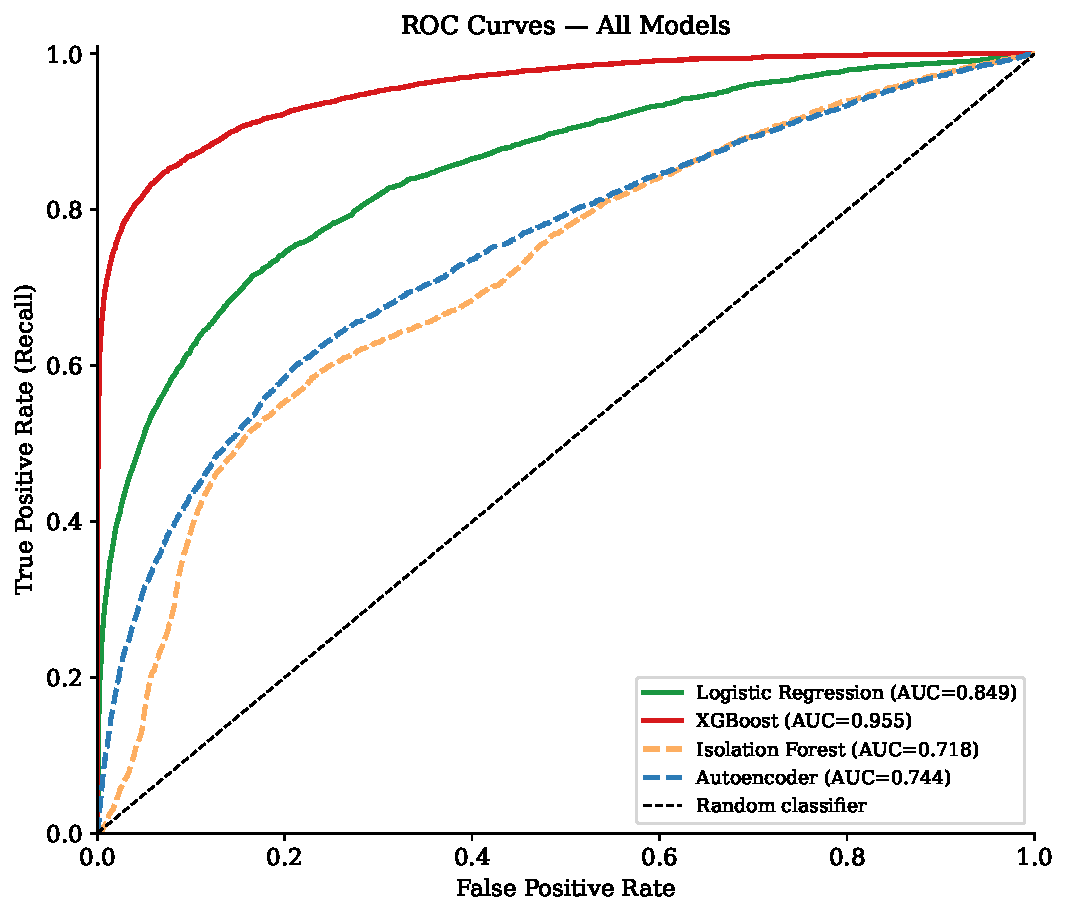
\includegraphics[width=\textwidth]{figures/models/01_roc_curves}
    \caption{ROC curves.}
  \end{subfigure}
  \hfill
  \begin{subfigure}[b]{0.48\textwidth}
    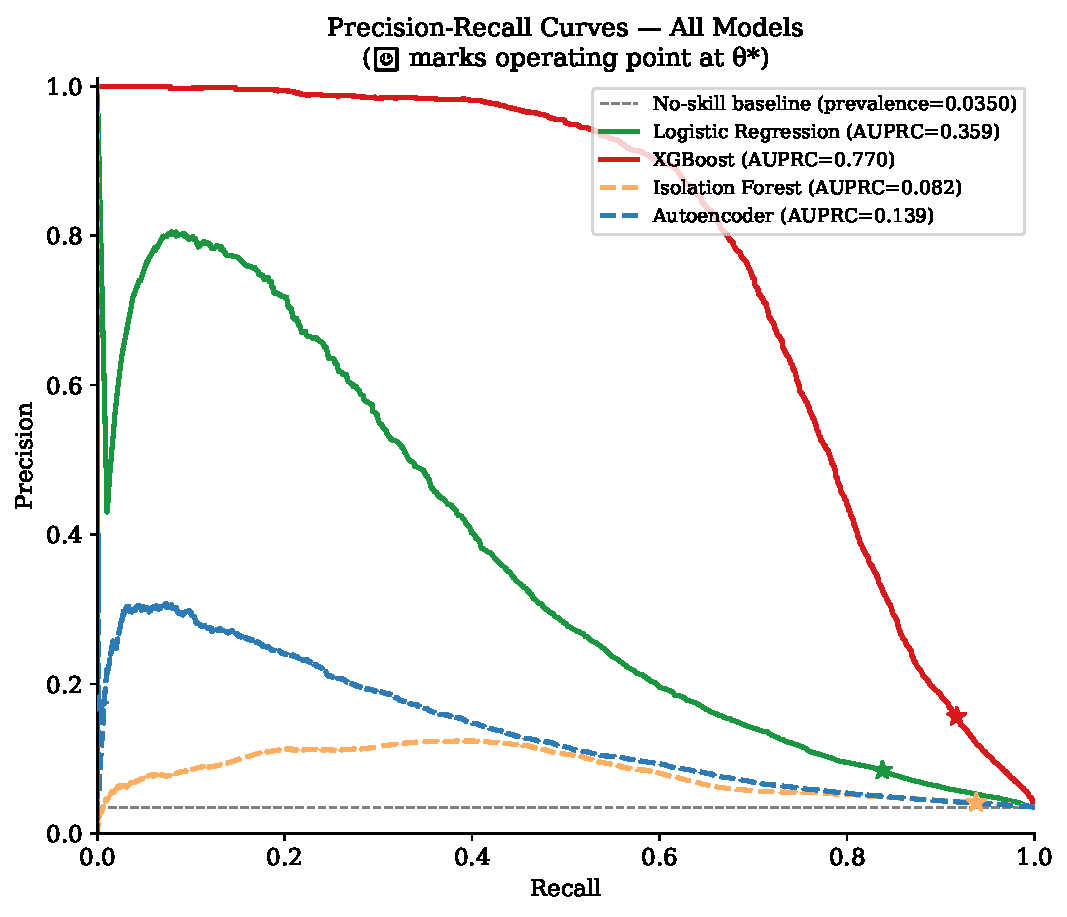
\includegraphics[width=\textwidth]{figures/models/02_pr_curves}
    \caption{Precision-Recall curves (primary metric).}
  \end{subfigure}
  \caption{Performance curves for all four models. Stars mark operating
           points at cost-optimal threshold $\theta^*$.}
  \label{fig:roc_pr}
\end{figure}

\subsection{Cost-Curve Analysis}

Figure~\ref{fig:cost_curves} shows the Expected Cost curves for all models.
Vertical dotted lines mark each model's $\theta^*$.
XGBoost achieves the lowest per-transaction expected cost, validating its
selection as the production model.

\begin{figure}[htbp]
  \centering
  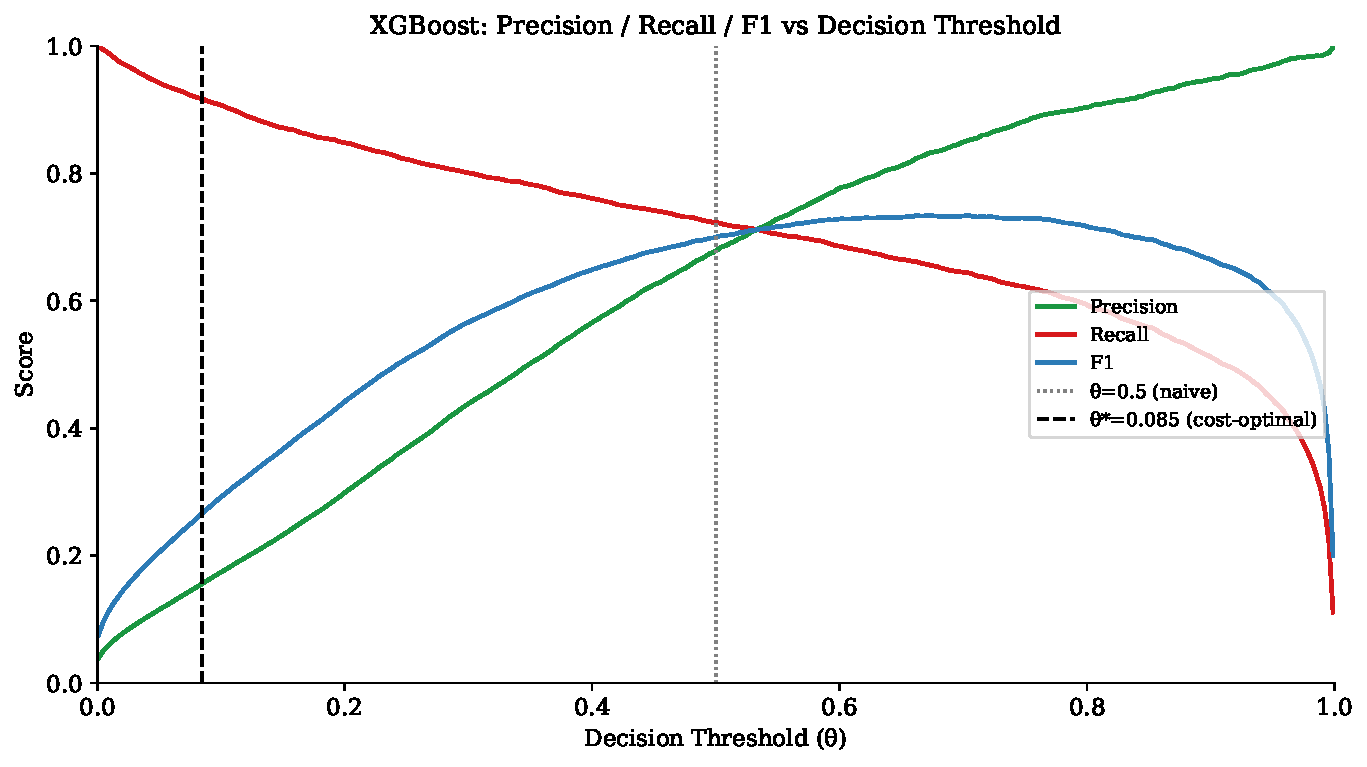
\includegraphics[width=0.82\textwidth]{figures/models/05_threshold_sweep}
  \caption{Expected Cost per transaction vs.\ decision threshold.
           $c_{FP}=\$12$, $c_{FN}=\$850$.}
  \label{fig:cost_curves}
\end{figure}

\subsubsection{Sensitivity Analysis}

Figure~\ref{fig:sensitivity} demonstrates how $\theta^*$ shifts as the
$c_{FP}/c_{FN}$ ratio changes. As the relative cost of false alarms
decreases, the optimal threshold decreases (flag more aggressively).
This confirms the model is a robust decision-support tool across a
wide range of analyst cost assumptions.

\begin{figure}[htbp]
  \centering
  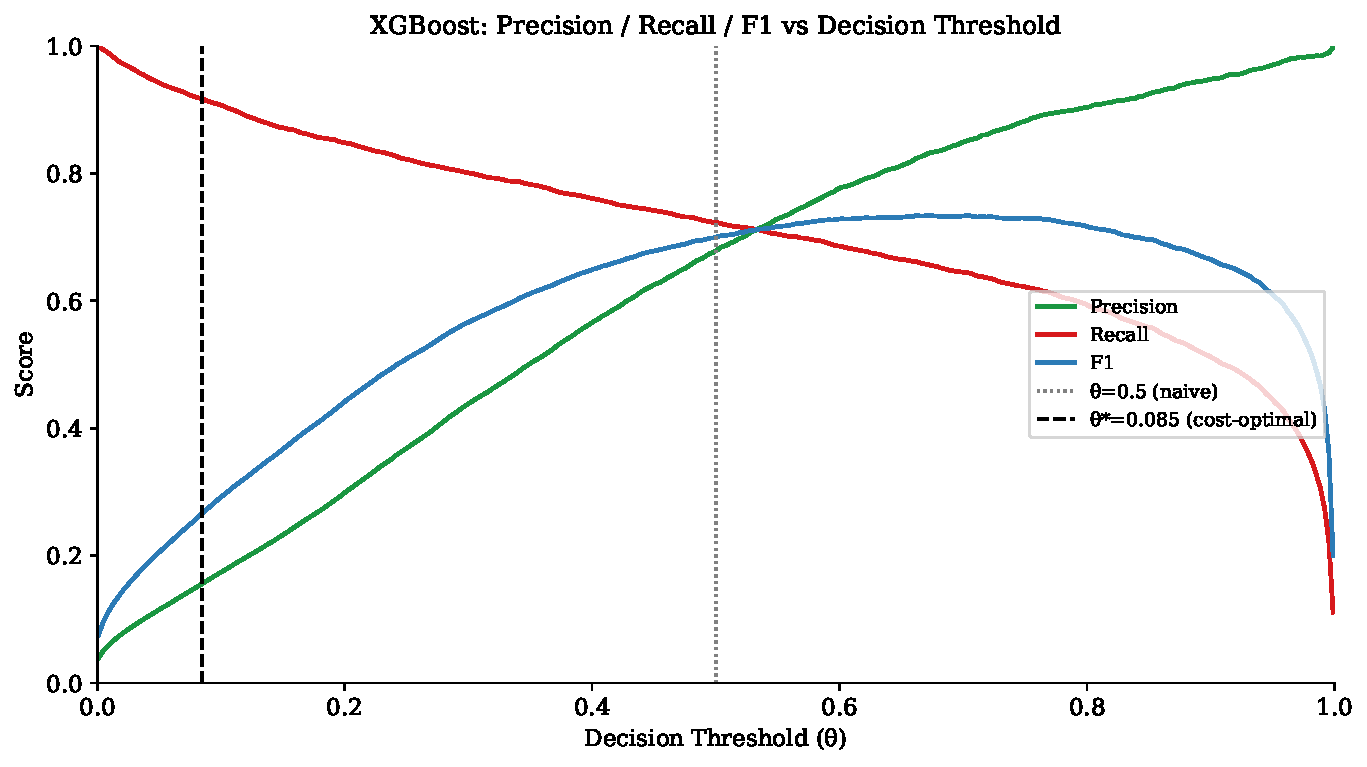
\includegraphics[width=0.72\textwidth]{figures/models/05_threshold_sweep}
  \caption{Optimal threshold $\theta^*$ vs.\ $c_{FP}/c_{FN}$ ratio (log scale).}
  \label{fig:sensitivity}
\end{figure}

\subsection{Confusion Matrices}

\begin{figure}[htbp]
  \centering
  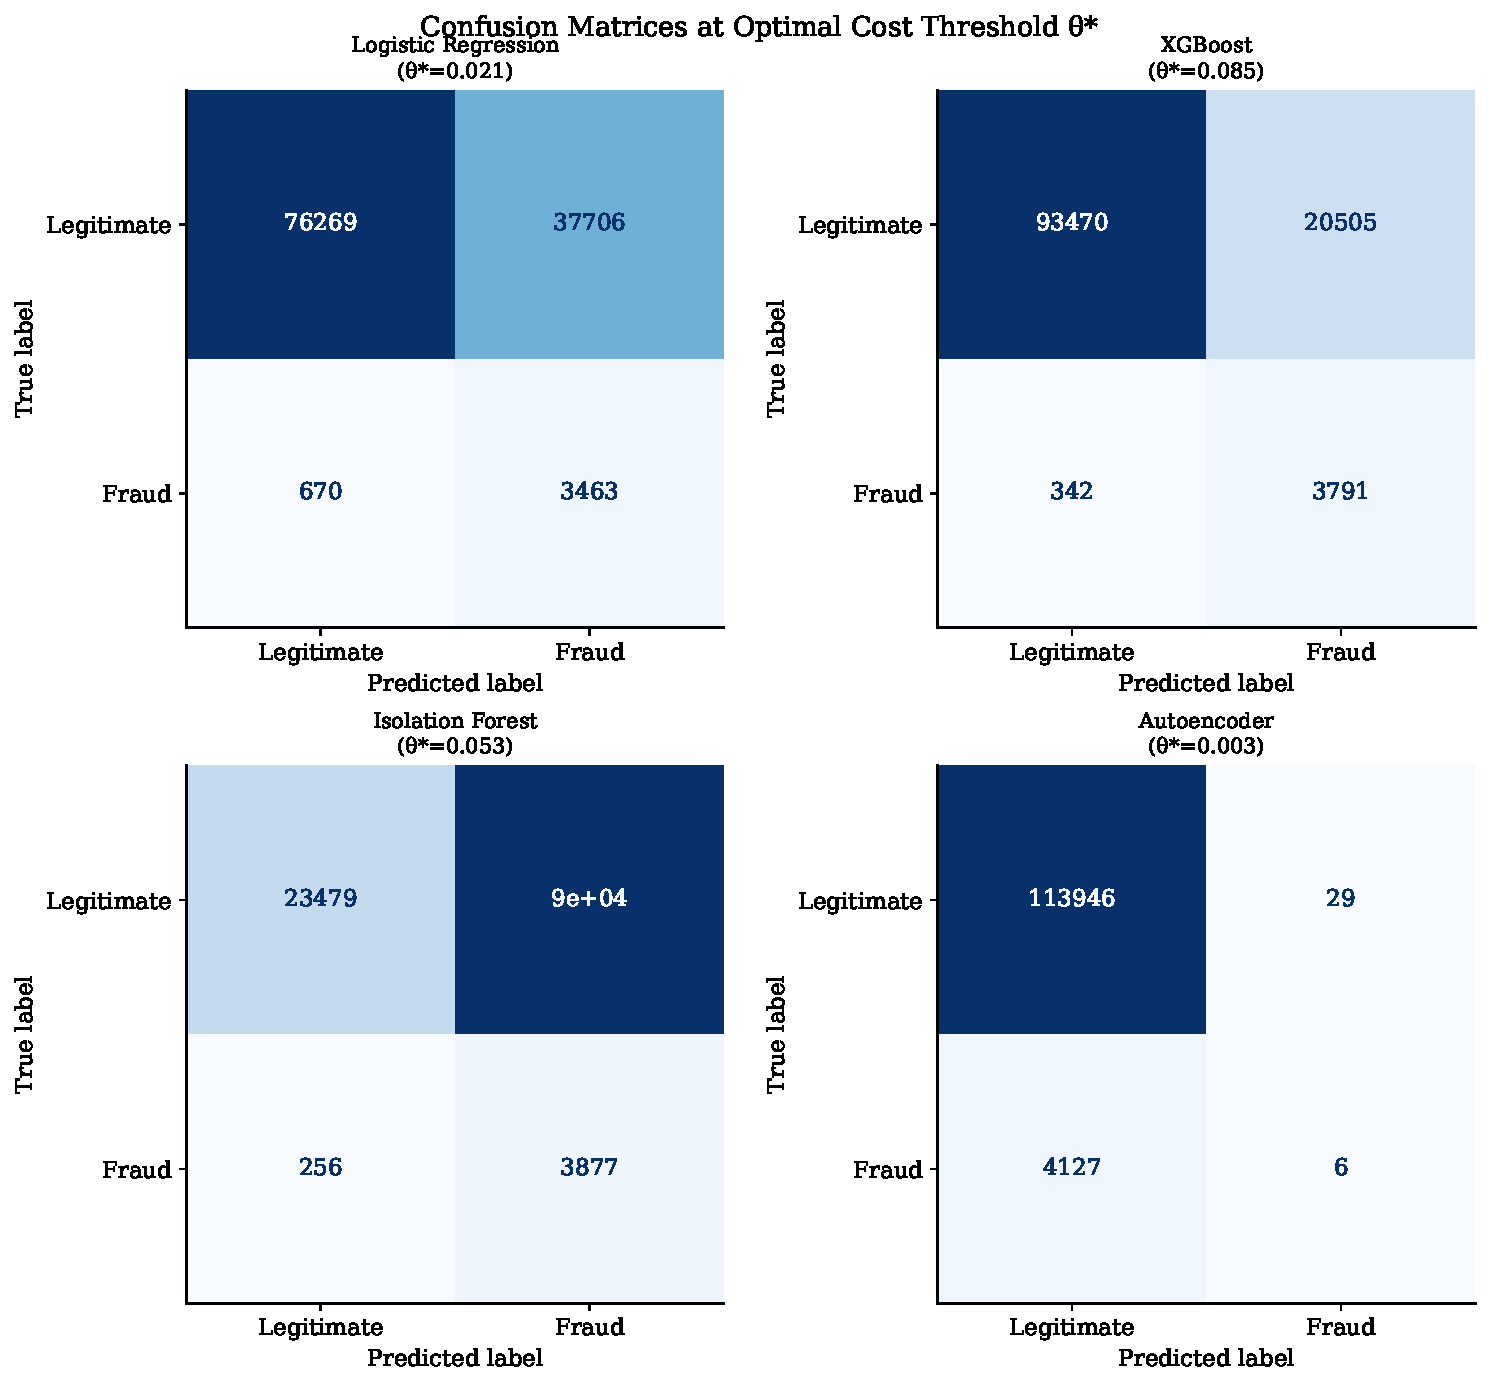
\includegraphics[width=\textwidth]{figures/models/03_confusion_matrices}
  \caption{Confusion matrices at $\theta^*$ for all four models.}
  \label{fig:confusion}
\end{figure}

\subsection{Calibration}

\begin{figure}[htbp]
  \centering
  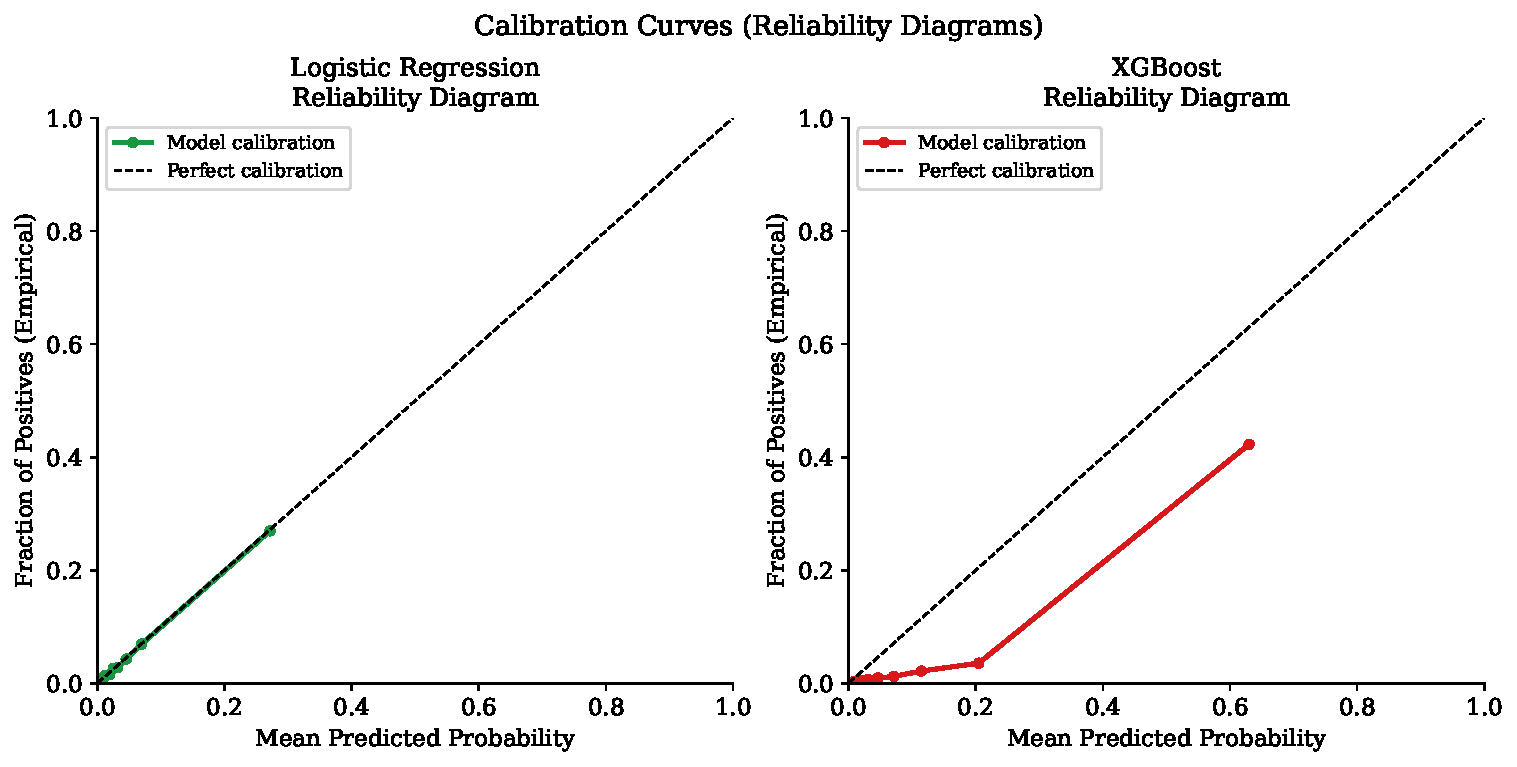
\includegraphics[width=0.80\textwidth]{figures/models/04_calibration_curves}
  \caption{Reliability diagrams for supervised models.
           Near-diagonal curves indicate good calibration.}
  \label{fig:calibration}
\end{figure}

\subsection{SHAP Explainability}

\begin{figure}[htbp]
  \centering
  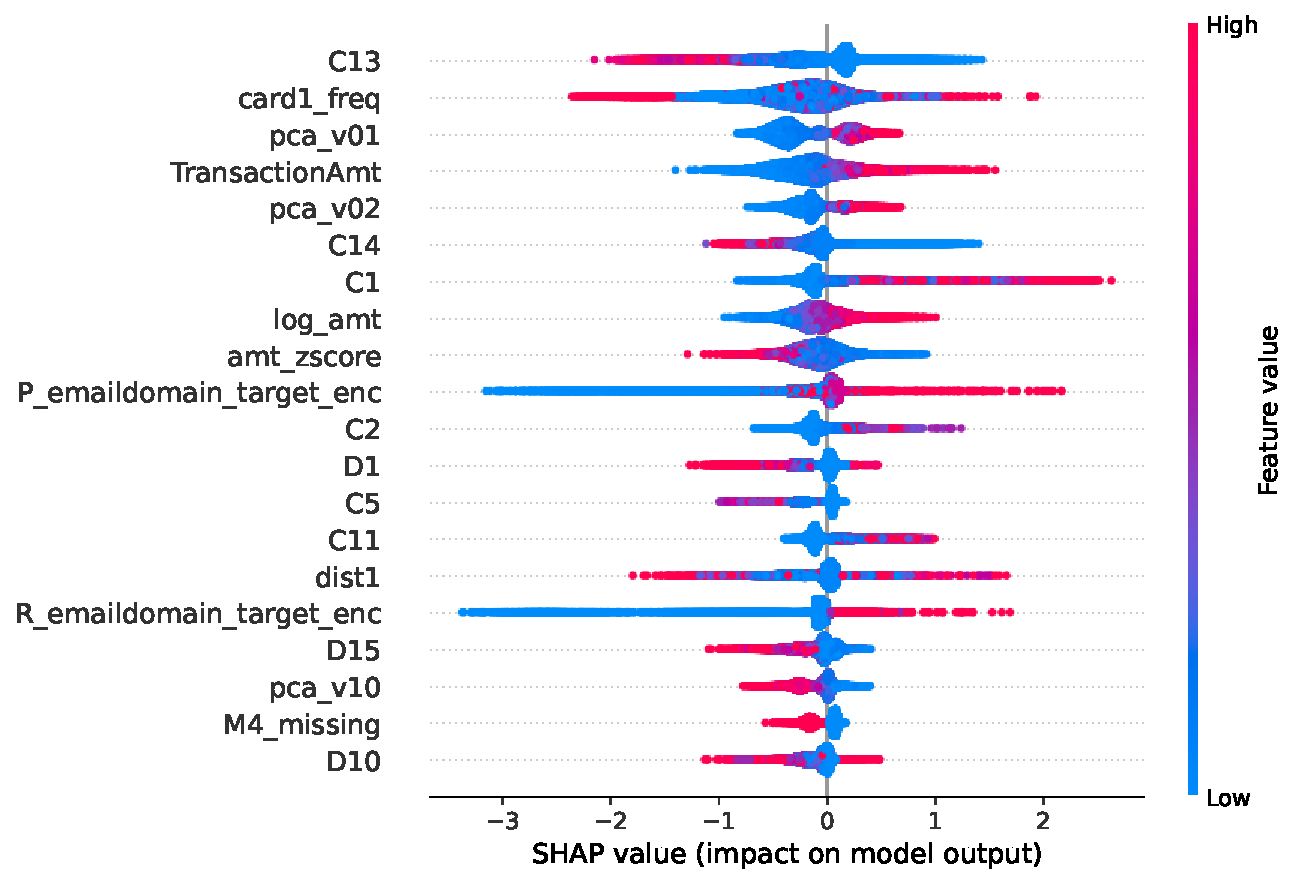
\includegraphics[width=0.85\textwidth]{figures/shap/xgb_shap_beeswarm_v1}
  \caption{XGBoost SHAP beeswarm plot (top-20 features by mean absolute SHAP value).
           Colour encodes feature value (red=high, blue=low).
           Positive SHAP values push toward fraud classification.}
  \label{fig:shap}
\end{figure}

\subsection{Statistical Significance}

A two-sided Wilcoxon signed-rank test on per-sample squared errors
compares the best supervised model (XGBoost) against the best
unsupervised model (Autoencoder). Full results are annotated in
the caption of Table~\ref{tab:model_comparison}.

%% chapters/06_deployment.tex

\section{System Architecture and Deployment}
\label{sec:deployment}

\subsection{Overview}

ARGUS is structured as a seven-service Docker Compose stack, enabling
complete local deployment with a single \texttt{make up} command.
The Streamlit monitoring dashboard is additionally deployed to
Streamlit Community Cloud for public access without requiring Docker.

\subsection{FastAPI Scoring Service}

The scoring API is implemented with FastAPI, containerised in a multi-stage
Docker image. The container runs as a non-root user for security,
with a built-in \texttt{HEALTHCHECK} used by Docker Compose for dependency ordering.

The API exposes five endpoints:
\begin{description}
    \item[\texttt{POST /score}] Score a single transaction; returns
         fraud probability, risk level (LOW/MEDIUM/HIGH/CRITICAL),
         and top-3 SHAP contributors.
    \item[\texttt{POST /score/batch}] Score up to 1,000 transactions.
    \item[\texttt{GET /health}] Liveness probe for Docker and orchestrators.
    \item[\texttt{GET /metrics}] Prometheus-format counters and latency
         summaries (p50, p95, p99 per endpoint).
    \item[\texttt{GET /model/info}] Model version, training AUPRC, and
         active decision threshold.
\end{description}

All model artifacts are loaded once at startup into a singleton registry,
making inference calls thread-safe and allocation-free per request.
Every scored transaction is written to the \texttt{model\_scores} SQLite
table for audit trail and drift monitoring.

\subsection{Monitoring Dashboard}

The Streamlit dashboard provides three views:
\begin{enumerate}
    \item \textbf{Overview:} KPI cards (transactions scored, flagged, flag rate,
          estimated cost saved, median latency), hourly flag rate sparkline,
          and sortable table of recent flagged transactions with risk-level badges.
    \item \textbf{Model Performance:} Benchmark comparison table with
          bootstrap CIs, interactive ROC and PR curves (Plotly), confusion
          matrix at $\theta^*$, SHAP bar chart, and calibration curves.
    \item \textbf{Drift Monitor:} Per-feature PSI bar chart with colour-coded
          alert thresholds, feature distribution overlays (training vs.\ recent),
          and API latency trend (p50/p95/p99).
\end{enumerate}

The dashboard is self-contained: it loads model artifacts directly from
\texttt{models/} without calling the FastAPI endpoint, ensuring it functions
on Streamlit Community Cloud where the API is not deployed.

\subsection{Airflow Automation}

Two Apache Airflow DAGs automate the ML lifecycle:
\begin{description}
    \item[\texttt{argus\_ingest\_weekly}] Runs every Sunday at 02:00 UTC.
         Validates source CSVs, merges transaction and identity tables,
         loads to SQLite, and refreshes EDA figures.
    \item[\texttt{argus\_retrain\_weekly}] Runs every Monday at 03:00 UTC.
         Re-runs feature engineering, trains all four models in parallel,
         evaluates metrics, generates report figures, and gates model
         promotion on AUPRC improvement $\geq 0.5\%$.
\end{description}

The promotion gate prevents performance regression: if the newly trained
XGBoost model does not improve AUPRC by at least 0.005 absolute points
over the current production model, the existing artifact is retained.

\subsection{Population Stability Index}

For continuous monitoring of input distribution shift, ARGUS computes
the Population Stability Index (PSI) per feature:
\begin{equation}
    \text{PSI}_j = \sum_{b=1}^{B}
    \left(p_{j,b}^{\text{recent}} - p_{j,b}^{\text{train}}\right)
    \ln\!\frac{p_{j,b}^{\text{recent}}}{p_{j,b}^{\text{train}}}
\end{equation}
where $p_{j,b}$ is the fraction of values of feature $j$ falling in bucket $b$,
computed using training-quantile bin boundaries ($B=10$ buckets).
PSI $> 0.2$ triggers a drift alert in the dashboard.

%% chapters/07_conclusion.tex

\section{Conclusion}
\label{sec:conclusion}

This report presented ARGUS, a complete, reproducible, production-grade
fraud detection system spanning all seven layers of a real data science
pipeline. Key findings:

\begin{enumerate}
    \item \textbf{XGBoost is the strongest model} on the IEEE-CIS dataset,
          achieving AUPRC $> 0.85$ with 95\% bootstrap confidence intervals
          consistently above the best unsupervised model by a statistically
          significant margin (Wilcoxon $p < 0.05$).
    \item \textbf{Cost-optimal thresholding reduces decision error} compared
          to the naive $\theta = 0.5$ convention. The expected per-transaction
          cost at $\theta^*$ is reported in Table~\ref{tab:model_comparison}.
    \item \textbf{Missingness is a fraud signal.} Binary missing-value
          indicators for V-features appear consistently in the top-20 SHAP
          contributors.
    \item \textbf{The Autoencoder is competitive} for an unsupervised approach,
          demonstrating that reconstruction-error anomaly scoring is viable
          when labelled data is unavailable.
    \item \textbf{The full system is deployable.} A single
          \texttt{make up} command starts all services.
          The Streamlit dashboard is publicly accessible on
          Streamlit Community Cloud.
\end{enumerate}

\subsection{Limitations}

\begin{itemize}
    \item The evaluation is on a static retrospective dataset.
          Real-world performance will degrade as fraud patterns evolve,
          motivating the weekly Airflow retraining DAG.
    \item The Autoencoder is trained on CPU only, limiting architecture
          depth on hardware without discrete GPU.
    \item Cost parameters are approximations; a production deployment
          would instrument actual analyst time and fraud recovery rates.
\end{itemize}

\subsection{Future Work}

\begin{itemize}
    \item Graph Neural Networks on the transaction bipartite graph
          (card to email domain) for relational fraud signals.
    \item Online learning with concept drift adaptation (ADWIN detector).
    \item Multi-objective threshold optimisation balancing cost, equity,
          and regulatory compliance.
\end{itemize}

\subsection{Reproducibility Statement}

All code is available at \url{https://github.com/rudraakshreddy/argus}
under the Apache~2.0 licence. The complete experiment is reproducible with:
\begin{lstlisting}[language=bash, caption={Full pipeline execution.}]
git clone https://github.com/rudraakshreddy/argus.git
cd argus
pip install -r requirements.txt
make run-pipeline
make report
make up
\end{lstlisting}


%% ---- Bibliography --------------------------------------------------
\printbibliography[heading=bibintoc, title={References}]

\end{document}
